\documentclass{article}
\usepackage[margin=3cm]{geometry}
\usepackage{textcomp}
\usepackage{graphicx}
\usepackage{float}
\usepackage{amsmath}
\usepackage[hidelinks]{hyperref}
\urlstyle{same}

\newcommand{\suppfignorm}{1}
\newcommand{\suppfigtotals}{2}
\newcommand{\suppfigorder}{3}
\newcommand{\suppfigbiophys}{4}

\title{When normalization gets prickly: are spike-ins good enough for single-cell RNA sequencing data?}
\author{Aaron Lun, Fernando Calero, Liora Vilmovsky, Bertie G\"ottgens, John Marioni}

\begin{document}

\maketitle

\section{Introduction}
Single-cell RNA sequencing (scRNA-seq) is a powerful technique for studying transcriptional activity in individual cells.
Briefly, RNA is isolated from single cells, reverse transcribed into cDNA and sequenced using massively parallel sequencing technologies \cite{shapiro2013singlecell}.
This can be done on microfluidics platforms like the Fluidigm C1 \cite{pollen2014lowcoverage}, or with protocols such as Smart-seq2 \cite{picelli2014full} that use microtiter plates.
Gene expression is quantified by mapping the read sequences to the genome and counting the number of reads mapped to each gene.
To avoid amplification biases, individual transcript molecules can also be tagged with unique molecular identifiers (UMIs) \cite{islam2014quantitative}, such that sequencing to saturation and counting UMIs will yield the number of transcripts of each gene in a cell.
Regardless of whether reads or UMIs are used, not all transcript molecules will be captured and sequenced due to cell-specific inefficiencies in reverse transcription \cite{stegle2015computational}.
The presence of these cell-specific biases compromises the direct use of the read/UMI count as a quantitative measure of gene expression.
Normalization is required to remove these biases before counts can be meaningfully compared between cells.

A common normalization strategy for RNA-seq data uses a set of genes that have constant expression across cells.
This set can consist of pre-defined ``house-keeping'' genes, or it can be empirically defined under the assumption that most genes are not differentially expressed (DE) between cells \cite{lun2016pooling,anders2010differential,robinson2010tmm}.
Counts are scaled to eliminate differences in the coverage of this non-DE set across cells.
Here, the assumption is that these differences between cells must be technical in origin, e.g., due to differences in library size or composition bias \cite{robinson2010tmm}.
Downstream analyses are then applied to the scaled counts to avoid obtaining misleading results.
This gene-based approach works well for bulk sequencing experiments where the population-wide gene expression profile is stable.
However, it may not be suitable for single-cell experiments where the presence of strong biological heterogeneity complicates the identification of a reliable non-DE set. 
For example, house-keeping genes may be turned on or off by transcriptional bursting, while cell cycling and other processes may trigger large-scale changes in the transcriptional programme that preclude the assumption of a non-DE majority.

An alternative normalization strategy uses spike-in RNA for which the identity and quantity of all transcripts is known \cite{stegle2015computational}.
The same amount of spike-in RNA is added to each cell, and the spike-in transcripts are processed along with their endogenous counterparts into a sequencing library.
This yields a set of read (or UMI) counts for both endogenous and spike-in transcripts in each cell.
Normalization is performed by scaling the counts for each cell such that the counts for the spike-in genes are, on average, the same between cells.
The central assumptions of this approach are that (i) the same amount of spike-in RNA is added to each cell, and (ii) the spike-in and endogenous transcripts are similarly affected by cell-to-cell fluctuations in capture efficiency.
Under these assumptions, any differences in the coverage of the spike-in transcripts between cells must be artifactual in origin and should be removed by scaling.
One particular advantage of this strategy is that it does not make any assumptions about the endogenous expression profile, unlike the non-DE approach described above.
This means that spike-in normalization can be applied in situations where large-scale changes in expression (e.g., related to changes in total RNA content) are expected and of interest \cite{lun2016stepbystep}.

However, there are several criticisms of spike-in normalization that challenge the validity of its central assumptions.
The first is that the same quantity of spike-in RNA may not be consistently added to each sample \cite{robinson2010tmm}, while the second is that synthetic spike-in transcripts may not behave in the same manner as endogenous transcripts \cite{grun2015design}.
Any differences in spike-in quantity or behaviour across cells will compromise the accuracy of spike-in normalization \cite{risso2014normalization}.
This would complicate the analysis of data sets where a non-DE majority cannot be assumed -- if spike-in normalization cannot be used, there is no obvious alternative for removing cell-specific biases.
However, whether or not the aforementioned criticisms are valid in real scRNA-seq experiments is yet to be determined.

In this paper, we conduct a series of experiments to estimate the reliability of spike-in normalization in single-cell transcriptome studies employing plate-based protocols.
We use mixtures of two distinct spike-in RNA sets to quantify the variance of the added spike-in volume across cells.
We also estimate the variability in differential behaviour between the sets, to determine how cell-specific biases change between different RNA populations.
Both factors are quantitatively negligible and have only minor effects on the results of downstream analyses such as detection of DE and highly variable genes.
These results suggest that spike-ins can be safely used for routine normalization of scRNA-seq data.

% The advantage of spike-ins is that it can capture cell size and doesn't require a non-DE majority.
% However, is the cell size interesting, or should it be normalized out (in which case accurate spike-in addition wouldn't be required at all)?
% It's most obviously useful for cell cycle considerations -- possibly also cancer and in some aspects of differentiation.
% The Islam non-UMI dataset is one example where there seems to be a 20-50-fold increase in counts in the MEFs vs mESCs.
% 
% I guess spike-in normalization is more technically correct, even if you end up getting every gene as being DE (technically true in terms of molecules, but possibly irrelevant).
% Rankings definitely change - spike-in normalization would favour genes that are upregulated on top of an increase in RNA content (as these would be hugely significant).
% Standard normalization would have no preference as you seek the balance between the two extremes.
% On the other hand, any non-DE genes with no change in the molecule number will be called as significant in standard normalization, which is definitively wrong.
% You could have your cake and eat it by separating the DE list into up/down changes for easier examination of the up/down changes.

\section{Results}

\newcommand\variance{\mbox{var}}

\subsection{Overview of the mixture experiments}
We aimed to assess the variability in the added spike-in quantity across cells.
To do so, we performed mixture experiments using two distinct spike-in sets (Figure~\ref{fig:expdesign}) -- the External RNA Controls Consortium (ERCC) set and the Spike-in RNA Variants (SIRV) set.
An equal volume of each spike-in set was added separately to a single well of a 96-well microtiter plate.
Each well also contained a single mouse cell (416B cells or trophoblasts) to mimic real experimental conditions.
The resulting pool of endogenous/spike-in RNA in each well was used to generate a library with the Smart-seq2 protocol.
This process was repeated for multiple wells and sequencing was performed on all libraries.

\begin{figure}[tbp]
\begin{center}
\includegraphics[width=0.8\textwidth]{pics/plate_setup.pdf}
\end{center}
\caption{Schematic of the experimental design to assess the variability of spike-ins in a plate-based scRNA-seq protocol.
(a) A cell is sorted into each well of a plate and lysed.
For one set of wells, an equal volume of each spike-in set is added separately into each well during the reverse transcription (RT) step.
For a different set of wells, an equal volume of a pooled mixture of the two spike-ins is added into each well, again during the RT step (done twice for consistency).
PCR amplification, library generation and sequencing is then performed.
(b) The log-ratio between the total counts of the two spike-in sets is computed for each well.
The variance of the log-ratio is estimated from all wells with separate addition of spike-ins, and from wells with addition of the premixed pool.
The difference between these two variance estimates represents the variance attributable to volume addition.
}
\label{fig:expdesign}
\end{figure}

For each library, reads were mapped to the genome and assigned to genes to quantify expression.
The total count was computed across all transcripts of each spike-in set in each well.
The log-ratio of the totals between the two sets was computed for each well, and the variance of this log-ratio was computed \textit{across} wells.
Any variability in spike-in volume addition should manifest as an increase to the variability of the log-ratio, given that the spike-in sets were added independently to each well.

We also repeated the experiment by adding volumes of ``premixed'' spike-in solution where the two spike-in sets had been pooled at a 1:1 ratio.
This ensures that there is no well-to-well variability in the relative quantities of RNA from the two spike-in sets.
The variance of the log-ratio across these premixed-addition wells provides a baseline level of variability in the protocol (e.g., due to sequencing noise).
The variance of volume addition was then estimated as the difference in the variance estimates from the premixed-addition wells and from the wells with separate addition of spike-ins.
We performed both the premixed and separate-addition experiments on the same plate to avoid plate effects.

We used a protocol based on microtiter plates rather than microfluidics as it is easier to customise the spike-in addition step in the former.
Our experimental design requires two separate additions of spike-in RNA to each reaction (see Methods).
This is not straightforward to achieve on, say, the Fluidigm C1 chip where the added volume for each reagent depends on the design on the reaction chamber.
Plate-based protocols also tend to be cheaper and are compatible with existing laboratory techniques such as indexed fluorescently-activated cell sorting (FACS).
Thus, we focus on normalization of data from plate-based protocols, to reflect their increasing use in single-cell studies (CITE).

\subsection{Estimating the variance of volume addition}
Denote the log-transformed total count for well $i$ and spike-in set $s$ as
\[
T_{is} = \log \left[ L_i V_{is} R_{is} \sum_{t_s} r_{t_s} c_{t_s} \right] + \varepsilon_{is}
\]
where $c_{t_s}$ is a constant specifying the concentration (in terms of transcripts per unit of volume) of each spike-in transcript $t_s$;
$r_{t_s}$ is a constant specifying the optimal transcript molecule-to-cDNA fragment capture rate for $t_s$;
$R_{is}$ is a random variable representing the average capture efficiency in well $i$ for all transcripts in set $s$, ranging from 0 to 1 and scaling $r_{t_s}$ to determine the actual capture rate for each $t_s$;
$V_{is}$ is a random variable representing is the volume of solution for $s$ added to $i$;
$L_i$ is the library-specific scaling factor for converting the number of fragments to that of reads, accounting for, e.g., library size and composition biases;
and $\varepsilon_{is}$ is the error term attributable to sequencing noise and variability in library preparation, where $\variance(\varepsilon_{is})= \sigma^2_{lib(s)}$.
We assume that $R_{is}$, $V_{is}$ and $\varepsilon_{is}$ are mutually independent of each other, and that $V_{is}$ and $\varepsilon_{is}$ for different $s$ are independent.

Let $s=1$ represent the ERCC spike-in set and $s=2$ represent the SIRV spike-in set.
In the experiment where each spike-in set is added separately to each well, denote the log-ratio of the total counts between the two sets as $\theta_i = T_{i1} - T_{i2}$ for well $i$.
This can also be written as
\[
\theta_i = \log V_{i1} + \varepsilon_{i1} - \log V_{i2} - \varepsilon_{i2} + R_i
\]
where $R_i = \log(R_{i1}/R_{i2})$ and represents the fold change in the average capture efficiency between the two sets (i.e., the difference in behaviour of the spike-ins).
Computing the variance of $\theta_i$ yields
\[
\variance(\theta_i) = 2 \sigma^2_{vol} + \sigma^2_{lib(1)} + \sigma^2_{lib(2)} + \variance(R_i)
\]
where $\sigma^2_{vol}$ is the variance of $\log V_{i1}$ and $\log V_{i2}$.
The volume addition procedure is the same for each spike-in set, so $V_{i1}$ and $V_{i2}$ should have the same distribution.
Also, we consider the variance of $R_i$ because $R_{i1}$ and $R_{i2}$ are not independent, e.g., due to well-specific effects on capture efficiency.

In the experiment where the spike-in sets are premixed before addition, $V_{i1}=aV_{i2}$ for some constant $a$ representing the proportions in which the two sets are mixed.
(This should be close to unity.)
If the same premixed solution is added to each well, the relative volume of ERCC spike-ins to SIRV spike-ins must be constant for all wells.
This means that the log-ratio for the premixed experiment becomes
\[
\theta'_i = \log a + \varepsilon_{i1} - \varepsilon_{i2} + R_i \;.
\]
As $a$ is constant for all $i$, the variance of $\theta'_i$ is
\[
\variance(\theta'_i) = \sigma^2_{lib(1)} + \sigma^2_{lib(2)} + \variance(R_i) \;.
\]
This represents the technical variance attributable to the rest of the scRNA-seq protocol.
To obtain an estimate of the variance of the volume addition step, simple arithmatic yields
\[
\sigma^2_{vol} = \frac{\variance(\theta_i) - \variance(\theta'_i)}{2} \;.
\]
It should be stressed that this variance estimate is relevant to all experiments using the same protocol for spike-in addition, even if the identity or concentration of the spike-in set is different.

Using this mathematical framework, we proceeded to estimate the variance components from the data from our mixture experiments.
We observed that the log-ratios $\theta_i$ and $\theta'_i$ computed from each plate were roughly normally distributed (Supplementary Figure~\suppfignorm{}).
Thus, we fitted a linear model to each set of log-ratios and used the residual variance of the fit as our variance estimate.
This allows blocking on additional structure in the experimental design (Methods).
We also noted that the distribution of $T_{is}$ was similar between separate-addition and premixed-addition wells within each plate (Supplementary Figure~\suppfigtotals{}).
This means that we do not need to consider complex mean-variance relationships when comparing variance estimates, i.e., the contribution of $\sigma^2_{lib(s)}$ will not change between $\variance(\theta_i)$ and $\variance(\theta'_i)$ for each plate.
Finally, we performed additional controls where we reversed the order of addition, i.e., SIRV spike-ins were added before the ERCC spike-ins.
In general, the order did not affect the variance estimates for the separate-addition wells (Supplementary Figure~\suppfigorder{}).

Our results indicate that $\sigma^2_{vol}$ is consistently smaller than the variance in the rest of the protocol (Figure~\ref{fig:varestimates}).
Indeed, no significant difference was detected between $\variance(\theta_i)$ and $\variance(\theta'_i)$ for each plate.
This indicates that variability of spike-in volume addition is a minor contributor to the technical variability of the spike-in counts.
To further put these estimates into context, consider that $T_{is}$ represents the log-transformed ``size factor'' for the library generated from well $i$.
In other words, all counts in this library are scaled by $\exp(-T_{is})$ to correct for well/cell-specific biases during spike-in normalization.
The variance of the log-size factors is several orders of magnitude larger than $\sigma^2_{vol}$.
This suggests that the latter will not have a major effect on the outcome of spike-in normalization.

\begin{figure}[btp]
    \begin{center}
        \includegraphics[height=2.2in,trim=0mm 10mm 0mm 10mm,clip]{../real/pics/variance_exp.pdf}
        \includegraphics[height=2.2in,trim=0mm 10mm 0mm 10mm,clip]{../real/pics/variance_sf.pdf}
    \end{center}
    \caption{Variance estimates of the log$_2$-ratio between the ERCC and SIRV total counts (left), or the log-size factors computed from those totals (right).
        Estimates were defined as the residual variance of a linear model fitted to the log-ratios or log-size factors across all cells (416B or trophoblasts) in each plate.
        Error bars represent the standard errors of the estimates, assuming normally-distributed values.
    }
    \label{fig:varestimates}
\end{figure}

\subsection{Estimating the variance of capture efficiency}
The variance of $R_i$ is also relevant as it determines the effect of differences in behaviour between distinct sets of transcripts.
Even when the capture efficiency differs between sets, spike-in normalization may still be appropriate \textit{provided that the fold change in capture efficiency is the same in all wells}.
Consider a situation where there is a consistent increase in efficiency in the spike-in set relative to endogenous transcripts.
This scales up the counts for the spike-in transcripts in all libraries by the same amount, which cancels out between libraries (i.e., the fold changes between counts for endogenous or spike-in transcripts in different libraries are unaffected).
However, if the fold change in efficiency varies across wells, the accuracy of spike-in normalization is compromised.
This is because changes in the capture efficiency for the spike-in transcripts are confounded with changes in efficiency for all transcripts in the well, precluding the use of spike-ins to normalize the counts for the endogenous trancripts.

In our mathematical framework, the estimated variance of $\theta'_i$ provides an upper bound for the variance of $R_i$.
This quantifies the extent to which normalization is affected by differences in efficiency between two transcript sets.
We observe that $\variance(\theta'_i)$ is an order of magnitude lower than the variance of the log-size factors in each plate (Figure~\ref{fig:varestimates}).
This indicates that the variance in efficiency across wells, while greater than $\sigma^2_{vol}$, is still relatively small compared to the other factors driving normalization, e.g., differences in cellular RNA content, well-to-well variability in capture efficiency for all transcripts.
Obviously, $R_i$ is computed between two spike-in sets whereas the differences between synthetic spike-in and endogenous transcripts are likely to be greater.
Nonetheless, the SIRV and ERCC spike-ins do vary in their biophysical properties (Supplementary Figure~\suppfigbiophys{}).
For example, the SIRV transcripts have more variable length and lower GC content compared to the ERCC transcripts.
This suggests that $R_i$ will include some of the differences in behaviour between synthetic and endogenous RNA, such that $\variance(R_i)$ can be used as a rough estimate of the magnitude of the associated variability.

\subsection{Assessing the downstream effect of variability with simulations}
We assessed whether the results of downstream analyses were sensitive to spike-in variability, especially for those analyses that depend on the assumption of constant spike-ins for normalization.
Simulations were prepared from real data sets containing counts for spike-in transcripts.
Specifically, the added volume and relative capture efficiency of spike-ins for each well were resampled and the spike-in counts were rescaled to reflect this new volume/efficiency.
The results of the analysis on the simulated data were then compared to the original results.
Any changes indicate that the analysis is sensitive to spike-in variability.
The advantage of this approach is that it only modifies the scale of the spike-in counts -- the counts for the cellular genes are used directly and do not need to be simulated.
The variance of the sampling distribution for the volume/efficiency is also based on the experimental estimates of spike-in variance.
This ensures that sensitivity will be assessed under realistic conditions. 

\section{Discussion}

\section{Methods}

\subsection{Spike-in mixture experiments with Smart-seq2}
% On a single plate, so no plate effects.
% Mention cutting up of plate, especially for the two conditions.
% No effect of different cell treatments.

\subsection{Data analysis for the mixture experiments}
Reads were mapped to the mm10 build of the mouse genome with additional sequences for transcripts in the ERCC (\url{https://tools.thermofisher.com/content/sfs/manuals/ERCC92.zip}) and SIRV (\url{https://www.lexogen.com/wp-content/uploads/2015/11/SIRV_Sequences_151124.zip}) spike-in sets.
Mapping was performed using the subread aligner v1.5.0 \cite{liao2013subread} in single-end RNA-seq mode with only unique alignments being retained.
Reads with mapping qualities greater than or equal to 10 were counted into exonic regions of genes using the featureCounts function in the Rsubread package v1.20.1 \cite{liao2014featurecounts}.
This was performed using the NCBI GRCm38 mouse annotation along with the annotation for the ERCC and SIRV transcripts, to obtain a count for each endogenous and spike-in gene in each well.

In each well, the sum of counts across all transcripts in each spike-in set was computed.
The log$_2$-ratio between the count sums of the ERCC and SIRV sets was calculated.
To estimate $\mbox{var}(\theta_i)$, a linear model was fitted to the log-ratios for all wells where the two spike-in sets were added separately.
This used a one-way layout where each combination of treatment (control or oncogene-induced) and spike-in addition order (ERCC or SIRV first) was treated as a separate group.
The variance was estimated as the mean of the squared residual effects.
This was repeated for $\mbox{var}(\theta_i')$ using all wells where premixed spike-ins were added.
Here, the model only contained two groups as addition order was irrelevant.

Variance decomposition was performed as described in Section~1 of the Supplementary Materials using the above estimates.
To determine the variability of $\psi_i$, each spike-in set was partitioned into two roughly similar halves.
This was done by sorting all transcripts in each set by their average counts; assigning all odd-ranked transcripts to one half; and assigning the remaining transcripts to the other half.
The log-ratios between the sums of the two halves were then used to estimate $\mbox{var}(\log \psi_i)$.

\subsection{Simulation design for resampling spike-in variability}
For each data set, the sum of the spike-in counts (referred to here as the spike-in total) was computed for each cell.
The variance of the log$_2$-transformed spike-in totals across cells includes sampling noise during library preparation or sequencing, variability in sequencing depth, and the variance of spike-in addition and capture efficiency between wells.
The final component (denoted here as $s^2$) represents spike-in variability and must be removed prior to simulation.
Otherwise, resampling will introduce variance for addition/efficiency on top of what is already present, leading to overrepresentation of $s^2$ in the variance of the simulated totals.
Removal was achieved by scaling the log$_2$-totals such that the variance across wells was reduced by $s^2$ without changing the mean.
The scaled log-values were then transformed back to ``processed'' totals that contain no variability due to addition or behaviour.

Simulations were performed by sampling a new value for the combined addition/efficiency effect in each cell.
Specifically, the effect for each cell was sampled independently from a $2^X$ distribution where $X \sim \mbox{Normal}(0, s^2)$.
This was used to scale the processed total to obtain a simulated total for each cell.
Counts for individual spike-in transcripts were then scaled to reflect this new total in each cell.
In this manner, the variance due to addition or capture efficiency was re-incorporated into the variance of the simulated totals across cells.
Note that addition and efficiency do not have to be simulated separately as they have the same effects in this framework -- a decrease in the spike-in total due to a decrease in the added spike-in volume cannot be distinguished from that due to reduced capture efficiency.

To scale the counts, a quantile adjustment approach was used to preserve the empirical mean-variance relationship.
A generalized linear model (GLM) was fitted to the counts across all cells for each spike-in gene, using the mglmOneGroup function in edgeR \cite{mccarthy2012differential, robinson2010edgeR} with an all-intercept design matrix.
An abundance-dependent trend was also fitted to the NB dispersions across all spike-in genes using the estimateDisp function.
In both cases, the original (natural) log-totals were used as the offsets for all cells.
The fitted GLM value and dispersion for each gene were treated as the true parameters of the NB distribution used to sample the observed count in each cell.
The simulated mean count for each gene in each cell was computed by taking the exponential of the sum of the log-simulated total for that cell and the GLM coefficient for that gene.
This was used as the mean of a simulated NB distribution, using the same value for the dispersion.
The quantile of each original count in its true distribution was mapped to a quantile in the simulated distribution, using the q2qnbinom function \cite{robinson2008small}.
This new quantile was used as the simulated count for the corresponding gene and cell.

% For simplicity, we assume that sequencing is performed to saturation in each data set, e.g., like UMIs.
% Thus, variability in the added volume will directly translate to variability in the total spike-in count.
% It also means that we do not have to rescale the cellular counts to reflect variable undersampling.
% Doing so would be problematic, as direct scaling of the counts would distort the empirical mean-variance relationship of the count data.

% The estimation of the true parameters conditions on the observed spike-in totals, and doesn't make the assumption that spike-in totals are constant.
% For example, if it turned out that you added half the amount of spike-in to one well, it wouldn't distort the estimation of the (conditional) mean.
% Okay, maybe the trended dispersion would be a bit weird, because technical variability should depend on the amount of RNA, but some inaccuracy there is forgivable.

The value of $s^2$ was set based on the previously estimated value for $\sigma^2_{vol} + \mbox{var}(\log \psi_{i}) \approx 0.05$.
This ensures that a realistic variance is used when sampling spike-in volume and efficiency in each well.

\subsection{Implementation of downstream analyses}
For the DE analyses, two scRNA-seq data sets were obtained -- one from a study with mouse embryonic stem cells (mESCs) and fibroblasts \cite{islam2011characterization} and another from a study with root epidermal and root center \textit{Arabidopsis Thaliana} cells \cite{brennecke2013accounting}.
In each study, DE genes were detected between cell types using edgeR \cite{robinson2010edgeR,lund2012detecting} and monocle \cite{trapnell2014dynamics}.
The former represents methods designed for analyses of bulk RNA-seq data, while the latter represents specialized single-cell methods.
For each method, spike-in normalization was performed by scaling the counts such that the spike-in totals were the same between cells.
The set of DE genes in the original data was then identified at a FDR of 5\% (see Section~Y in the Supplementary Materials for implementation details of each method).
This was repeated for the simulated data, and the proportion of genes common to both the original and simulated sets was computed.
The proportion of common genes in the top set of 20-2000 genes with the smallest $p$-values was also computed between the original and simulated analyses.
This was repeated for 10 simulation iterations, and the average proportions across iterations were reported for each method.

For detecting highly variable genes (HVGs), three scRNA-seq data sets were obtained -- one from a study of mouse haematopoietic stem cells \cite{wilson2015combined}, one from a study of murine immune cells \cite{brennecke2013accounting} and another from a study of mESCs \cite{islam2014quantitative}.
In each data set, HVGs were detected using two approaches based on spike-ins (see Section~Y in the Supplementary Materials for implementation details of each method).
The first approach is based on the method of Brennecke \textit{et al.} \cite{brennecke2013accounting} where the squared coefficient of variation for each gene is tested for a significant increase above technical noise.
The top set of HVGs was identified as those genes with the smallest $p$-values.
The second approach examines the variance of the log-counts, which provides some more robustness against outlier expression patterns.
Here, the top set of HVGs was identified as those with the largest biological components of the variance.
For both methods, the top set of 20-2000 genes was compared between the original and simulated analyses.
This was repeated for 10 simulation iterations, and the average proportions across iterations were reported for each method.

For dimensionality reduction and clustering, a scRNA-seq data set was obtained from a study of mESCs cultured under different conditions \cite{kolod2015single}.
A PCA plot was constructed from the original log-counts after spike-in normalization.
This was repeated for each simulation iteration, and the position of each cell on the simulated plot was mapped back to the corresponding location on the original plot.
In this manner, the sensitivity of the cell placement to spike-in variability was assessed.
Hierarchical clustering was also performed on the normalized log-counts using Euclidean distances or rank correlations.
The stability of each cluster was assessed based on the number of occurrences of that cluster across simulation iterations.
See Section~Y in the Supplementary Materials for further implementation details.

{\small
\bibliography{refnorm}
\bibliographystyle{unsrt}
}

\end{document}
